\chapter{Historical Evolution}
\label{ch:history}

The models of Chapter~4 are usually presented as a design space, as though an
architect had surveyed the options and chosen.
The history is less tidy.
Each
model was a response to a specific difficulty, several were formalised only after
hardware implementing them had already shipped, and at least two widely deployed
specifications were subsequently found not to describe the machines they governed.
This chapter traces that history, because the argument this paper examines --- that
sequential consistency is too expensive --- was made at a particular moment under
particular assumptions, and those assumptions are visible only in context.

\begin{figure}[H]
\centering
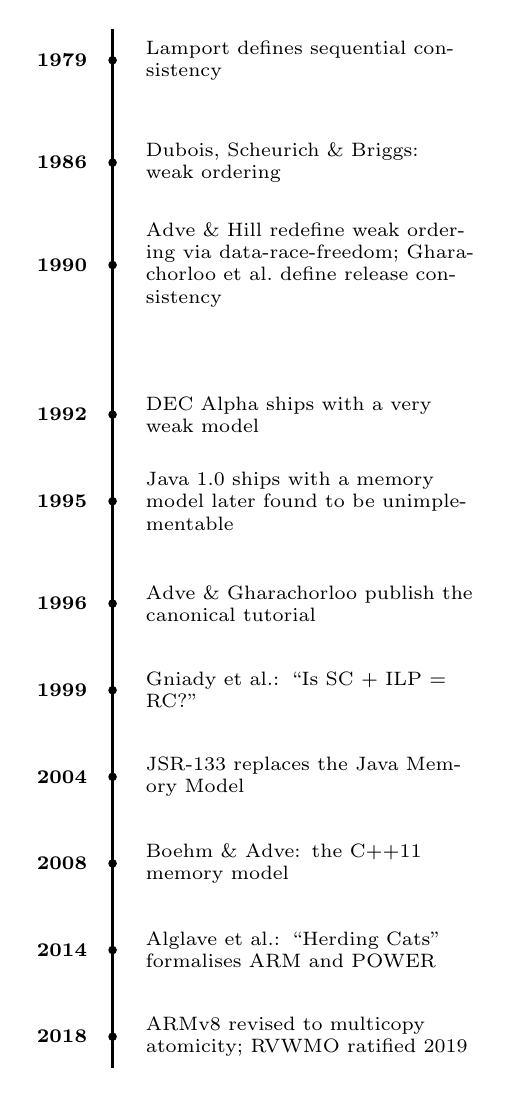
\begin{tikzpicture}[
    yr/.style={font=\scriptsize\bfseries},
    ev/.style={font=\scriptsize, align=left, anchor=west, text width=42mm},
    dot/.style={circle, fill=black, inner sep=1.1pt}]

  \draw[thick] (0,0) -- (0,-13.2);

  \foreach \y/\year/\text in {%
    -0.4/1979/{Lamport defines sequential consistency},
    -1.7/1986/{Dubois, Scheurich \& Briggs: weak ordering},
    -3.0/1990/{Adve \& Hill redefine weak ordering via data-race-freedom;
               Gharachorloo et al.\ define release consistency},
    -4.9/1992/{DEC Alpha ships with a very weak model},
    -6.0/1995/{Java 1.0 ships with a memory model later found to be unimplementable},
    -7.3/1996/{Adve \& Gharachorloo publish the canonical tutorial},
    -8.4/1999/{Gniady et al.: ``Is SC + ILP = RC?''},
    -9.5/2004/{JSR-133 replaces the Java Memory Model},
    -10.6/2008/{Boehm \& Adve: the C++11 memory model},
    -11.7/2014/{Alglave et al.: ``Herding Cats'' formalises ARM and POWER},
    -12.8/2018/{ARMv8 revised to multicopy atomicity; RVWMO ratified 2019}}
  {
    \node[dot] at (0,\y) {};
    \node[yr, anchor=east] at (-0.2,\y) {\year};
    \node[ev] at (0.3,\y) {\text};
  }
\end{tikzpicture}
\caption{Chronology of memory consistency models.}
\label{fig:timeline}
\end{figure}

\section{1979: The Definition}

Lamport's paper \cite{lamport1979multiprocessor} is three pages long and does not
argue that sequential consistency is desirable.
It assumes so, and asks what a
hardware implementation must satisfy to achieve it.
The two requirements it gives
--- each processor issues its requests in program order, and requests to a single
memory module are serviced in arrival order --- were, on the machines of 1979,
neither surprising nor expensive.
The paper is best read as a formalisation of
what everyone already believed the machine did.

The significance of the paper is that it made the assumption explicit and therefore
falsifiable.
Once SC had a definition, it became possible to build a machine that
demonstrably did not satisfy it, and to argue that doing so was a good idea.

\section{1986--1990: The Case for Relaxation}

Dubois, Scheurich and Briggs \cite{dubois1986memory} made that argument.
Their
observation was that SC's requirements bind at every memory operation, whereas
programs actually require ordering only at the few points where threads
communicate.
Enforcing ordering everywhere to protect the rare case is a poor
trade.
\emph{Weak ordering} follows: distinguish synchronisation accesses from
data accesses, and guarantee ordering only around the former.

Adve and Hill \cite{adve1990weak} reformulated this from the programmer's side.
Rather than defining weak ordering as a hardware behaviour, they defined it as a
\emph{contract}: if the programmer writes a data-race-free program, the hardware
will appear sequentially consistent.
This inversion is the single most consequential
idea in the field.
It made weak hardware defensible --- the programmer is not
exposed to reordering, provided the program is properly synchronised --- and it
supplied the framework in which every subsequent language-level memory model has
been written.

Gharachorloo et al.\ \cite{gharachorloo1990memory} refined it further with release
consistency, observing that acquire and release semantics need constrain only one
direction each, and so admit cheaper implementations than full barriers.

By 1990 the intellectual case was complete: SC is expensive, relaxation is safe for
well-written programs, and here is the framework proving it.
Hardware followed
immediately.
The DEC Alpha, designed in this period, adopted one of the weakest
models ever shipped.

\section{The Cost of Being Right}

The DRF settlement rested on a premise that received less scrutiny than it
deserved: that programmers would in fact write data-race-free programs.
The
subsequent three decades tested that premise.

\paragraph{Java, 1995 and 2004.} Java shipped in 1995 with a memory model intended
to give strong guarantees even to racy programs, for security reasons --- a
sandboxed language cannot let a race corrupt the virtual machine's own invariants.
The model was found to be simultaneously too weak to support the idioms
programmers used and too strong to permit standard compiler optimisations.
It was
replaced wholesale by JSR-133 \cite{manson2005java} after a multi-year effort.
That a memory model for a single language required nine years and a formal
committee is itself evidence about the difficulty of the subject.

\paragraph{C++, 2008.} C++ had no memory model at all until C++11. Multithreaded
C++ was written against the pthreads library, whose specification described
synchronisation but not the underlying memory semantics, leaving the correctness
of essentially all concurrent C++ formally undefined. Boehm and Adve
\cite{boehm2008foundations} supplied the missing foundation.

\paragraph{Specifications that did not describe the hardware.} Alglave, Maranget
and Tautschnig \cite{alglave2014herding} formalised the published ARM and POWER
architecture manuals and tested the resulting models against real processors.
The
models did not match: they permitted executions no chip produced and forbade some
that chips did.
The response, over the following years, included ARM's 2018
revision of ARMv8 to multicopy atomicity --- a \emph{strengthening} of a shipped
architecture, undertaken because the weaker model was too difficult to reason
about.

\section{1999--2011: The Counter-Argument}

While the industry moved right along the spectrum of Figure~\ref{fig:tension}, a
line of work asked whether it had needed to.

Gniady, Falsafi and Vijaykumar \cite{gniady1999sc} posed the question in their
title: \emph{Is SC + ILP = RC?} Their observation was that the 1980s cost estimate
for SC assumed the core would stall.
On a core that speculates, it need not: the
load may execute early and be squashed if a coherence invalidation proves the
speculation observable.
They reported that SC so implemented came close to release
consistency in performance.

Subsequent work extended the mechanism.
BulkSC \cite{ceze2007bulksc} abandoned
per-instruction reasoning in favour of executing large chunks of instructions
atomically, so that consistency is guaranteed at chunk boundaries --- the same
insight that underlies transactional memory.
InvisiFence
\cite{blundell2009invisifence} reduced the cost of the fences themselves.

Marino et al.\ \cite{marino2011sc} closed the remaining gap by addressing the
compiler, showing that a compiler forbidden from reordering shared memory accesses
loses only a few per cent of performance --- far less than had been assumed.

\section{The Unresolved Position}

The situation as it stands is peculiar.
The academic literature contains a
substantial body of evidence that sequential consistency can be implemented at
modest cost on a speculative core.
The commercial landscape contains no processor
that does so.
Meanwhile, ARM has strengthened its model, RISC-V's RVWMO was
ratified only after extended debate about how weak to make it, and the difficulty
of programming weak models is a matter of documented record rather than
speculation.

At least four explanations are available, and they are not mutually exclusive.

\begin{enumerate}
\item \textbf{The measurements do not scale.} The speculative-SC results were
  obtained at modest core counts.
Conflict frequency, and therefore squash rate,
  grows with cores.
\item \textbf{Energy, not time.} A squash discards completed work. In a
  power-constrained design --- which every mobile design is --- this may be
  decisive even where execution time is not.
\item \textbf{Verification.} Verifying a speculative implementation against a
  strong specification is substantially harder than verifying a straightforward
  implementation against a weak one.
\item \textbf{Architectural commitment.} A memory model is a permanent contract.
  Weakening one later is impossible; strengthening one, as ARM did in 2018, is
  possible but rare.
The safe choice for a vendor is to promise little.
\end{enumerate}

Distinguishing among these is beyond the scope of a single term paper, but the
first can be tested directly, and doing so is the purpose of the simulation study
described in the next chapter.
